
\documentclass[11pt,fleqn]{article}
\usepackage[margin=1in,top=1in,bottom=1in]{geometry}
\usepackage{mathtools}
\usepackage{longtable}
\usepackage{enumitem}
\usepackage{hyperref}
\usepackage[dvips]{graphics}
\usepackage[table]{xcolor}
\usepackage{amssymb}
\usepackage{subfig}
\usepackage{booktabs}
\usepackage{tikz}
\usepackage{pdflscape}

\usepackage[normalem]{ulem}

\usepackage{multicol}
\usepackage{txfonts}
%\usepackage{amsfonts}
\usepackage{natbib}

\usepackage{gb4e}
%\usepackage{/Users/judith/Library/Latex/drs}
%\usepackage{/Users/judith/Library/Latex/avm}
\usepackage[all]{xy}
\usepackage{rotating}
\usepackage{tipa}
\usepackage{multirow}
\usepackage{authblk}
\usepackage{adjustbox}
\usepackage{array}


\newcolumntype{R}[2]{%
    >{\adjustbox{angle=#1,lap=\width-(#2)}\bgroup}%
    l%
    <{\egroup}%
}
\newcommand*\rot{\multicolumn{1}{R{90}{1em}}}% no optional argument here, please!

\newcommand{\foc}{$_{\mbox{\small F}}$}
\newcommand{\lp}{<_{\hspace*{-.1cm}p}}
\newcommand{\lnai}{<_{\hspace*{-.1cm}nai}}

\setlength{\parindent}{.8cm}
\setlength{\parskip}{0ex}
\setlength{\headsep}{0in}

\setlength{\bibsep}{0mm}
\bibpunct[:]{(}{)}{;}{a}{,}{,}

\newcommand{\yi}{\'{\symbol{16}}}
\newcommand{\nasi}{\~{\symbol{16}}}
\newcommand{\hina}{h\nasi na}
\newcommand{\ina}{\nasi na}
%\renewcommand{\abut}{$\supset$\hspace*{-0.07cm}$\subset$}
\newcommand{\tto}{t$_{top}$}
\newcommand{\wtop}{w$_{top}$}
\newcommand{\tc}{t$_c$}
\newcommand{\schwa}{\begin{sideways}e\end{sideways}}

% Semantic brackets
%\newcommand{\iss}[1]{\mbox{\protect\tiny \mbox{#1}}}
%\newcommand{\sem}[2]{\6#1\9$_\iss{#2}$} David's original
\newcommand{\6}{\mbox{$[\hspace*{-.6mm}[$}} 
\newcommand{\9}{\mbox{$]\hspace*{-.6mm}]$}}
\newcommand{\sem}[2]{\6#1\9$^{#2}$}

\newcommand{\semt}[2]{$\left[\hspace*{-.6mm}\left[\begin{tabular}[c]{@{}l@{}}#1\vspace*{-.5em}\end{tabular}\right]\hspace*{-.6mm}\right]\hspace*{-.6mm}^{#2}$}

\renewcommand{\baselinestretch}{1}

\def\bad{{\leavevmode\llap{*}}}
\def\marginal{{\leavevmode\llap{?}}}
\def\verymarginal{{\leavevmode\llap{??}}}
\def\infelic{{\leavevmode\llap{\#}}}

\definecolor{Lighter}{gray}{.92}
\definecolor{Blue}{RGB}{0,0,255}
\definecolor{Green}{RGB}{10,200,100}
\definecolor{Red}{RGB}{255,0,0}


\newcommand{\citepos}[1]{\citeauthor{#1}'s \citeyear{#1}}
\newcommand{\citeposs}[1]{\citeauthor{#1}'s}
\newcommand{\citetpos}[1]{\citeauthor{#1}'s (\citeyear{#1})}

\newcommand{\eref}[1]{(\ref{#1})}
\newcommand{\tableref}[1]{Table \ref{#1}}
\newcommand{\figref}[1]{Fig.~\ref{#1}}
\newcommand{\appref}[1]{Appendix \ref{#1}}
\newcommand{\sectionref}[1]{section \ref{#1}}


\title{The influence of lexical meaning and prior belief on projectivity\thanks{This work was partially supported by NSF grant BCS-1452674 (JT).}}

\author{Judith and Judith}

%\author[$\bullet$]{Judith Tonhauser}
%\author[$\triangleright$]{Judith Degen}
%
%\affil[$\bullet$]{The Ohio State University}
%\affil[$\triangleright$]{Stanford University}

%\renewcommand\Authands{ and }
%
%\newcommand{\jt}[1]{\textbf{\color{blue}JT: #1}}
%\newcommand{\jd}[1]{\textbf{\color{Green}[jd: #1]}}  

\begin{document}

\maketitle

\begin{abstract}
Projective content, like presuppositions or conventional implicatures, is utterance content that a speaker may be taken to be committed to even when the expression associated with the content occurs embedded under an entailment-canceling operator (e.g., \citealt{ccmg90}). It has long been observed that non-entailed content may also be taken to be a commitment of the speaker when the expression associated with the content is embedded under such operators (e.g., \citealt{simons01,schlenker10,best-question}). Some authors, like \citealt{anand-hacquard2014}, assume that speaker commitment in such cases is a different phenomenon/should be given a different analysis (``illusion of factivity'' and ``illusion of projection''), whereas others, like \citealt{schlenker10} talks of ``part-time triggers''. Former authors assume that entailed content = presupposition, and non-entailed content = something else. Entailment is a binary property but is it really the way in which language users treat it?

The goal of this paper was to investigate whether projectivity is influenced by entailment and by the prior probability of the event described by the projective content.

We show that...and that....
\end{abstract}
			
\section{Introduction}\label{s1}

\begin{itemize}

\item \citealt*{tbd-variability} found that lexical content of projective content matters for projection.

\item Presuppositions are entailed content that is projective, i.e., that a speaker may be taken to be committed to even when the expression that the presupposition is associated with occurs under an entailment-canceling operator.

\item So projective content is often assumed to be entailed.

\item But we know that not only entailed content may be projective.

\item Entailment

\begin{itemize}

\item Entailment is a relation between two statements: A entails B if and only if every model in which A is true is also one in which B is true. 

A sentence (meaning) A entails B if whenever A is true, then B must also be true. 

Entailment is assumed to hold no matter what the facts of the world are.

\item \citealt[19f.]{ccmg90} ``A entails B =df whenever A is true, B is true \\ {[}...{]} \\  {\em A and not B} is contradictory (can't be true in any situation)''

\item \citealt{schlenker10}

\begin{exe}
\ex 
\begin{xlist}
\ex Context: Mary is a responsible 30-year old. 
\\ Mary has announced to her parents that she is pregnant. 
\\ it follows: Mary is pregnant \hfill (\citealt[139]{schlenker10})

\ex Context: Mary is playful 7-year old.
\\ Mary has announced to her parents that she is pregnant. 
\\ it does not follow: Mary is pregnant \hfill (\citealt[140]{schlenker10})

\ex John has announced that he has met Elvis
\\ it does not follow: John has met Elvis. \hfill (\citealt[140]{schlenker10})
\end{xlist}
\end{exe}

\end{itemize}

\end{itemize}

\section{Norming study: Prior probabilities of events}\label{s-norming}

\footnote{\label{f-github}The
data and R code for generating the figures and analyses
of the norming studies and the experiment reported on in this paper are available at \url{https://github.com/judith-tonhauser/projective-probability}.}

\subsection{Methods}\label{s-methods-1}

\paragraph{Participants.} 95 participants with U.S.\ IP addresses and at least 99\% of previous HITs approved were recruited on Amazon's Mechanical Turk platform (ages: 21-75; median: 33; 45 female, 50 male). They were paid 55 cents for participating in the experiment. 

\paragraph{Materials.} The prior probability of 20 events described by English sentences were explored in this experiment. Each of the 20 event descriptions was paired with two facts about the world, described by English sentences and labeled `Fact:', for a total of 40 fact/event pairs. Each event was hypothesized to be relatively more likely given one of the two facts than given the other fact that the event was paired with. Two fact/event pairs are given in (\ref{event}) for the event described by the English sentence {\em Mary is pregnant}: this event was hypothesized to be more likely given the fact described in (\ref{event1}i) than given the fact described in (\ref{event2}i). See Appendix \ref{a-exp1} for the other 19 event descriptions and the fact descriptions that the event descriptions were paired with.\footnote{Need to say that we use `event' for events and states, rather than `eventuality'.}

\begin{exe}
\ex\label{event}
\begin{xlist}
\ex\label{event1}
\begin{xlist}
\ex Fact: Mary is taking a prenatal yoga class
\ex Mary is pregnant
\end{xlist}
\ex\label{event2}
\begin{xlist}
\ex Fact: Mary is a middle school student
\ex Mary is pregnant
\end{xlist}
\end{xlist}
\end{exe}

{\bf fact/event pairs were chosen so that neither at ceiling nor at floor. We need to avoid eventualities being too likely or too unlikely, given their two facts, because a) if they are too likely, then people might argue that the facts of the world entail the content of the clause describing the eventuality, and b) if they are too unlikely, then participants might give wonky projectivity ratings.}

The experiment also included two control stimuli, which were used to assess whether participants were attending to the task. Like the target stimuli, both control stimuli consisted of a sentence describing a fact about the world and a sentence describing an event, as shown in (\ref{control1}) and (\ref{control2}). The two control stimuli differ in the probability of the event given the fact about the world: whereas the event of Barry living in Europe has a probability of 1, given the fact that Barry lives in Germany, the event of Tammy speaking Italian and Greek has a probability of 0, given that Tammy is a rabbit. 

\begin{exe}
\ex\label{control1}
\begin{xlist}
\exi{i.} Fact: Barry lives in Germany 
\exi{ii.} Barry lives in Europe 
\end{xlist}
\ex\label{control2}
\begin{xlist}
\exi{i.} Fact: Tammy is a rabbit 
\exi{ii.} Tammy speaks Italian and Greek 
\end{xlist}
\end{exe}

The 40 target stimuli were distributed across two lists of 20 target stimuli each so that each list contained 20 unique event descriptions and each list included 10 fact/event pairs for which the event was hypothesized to be likely and 10 fact/event pairs for which the event was hypothesized to be less likely. The two control stimuli were added to each list, for a total of 22 stimuli per list. 

\paragraph{Procedure.} Participants were randomly assigned to a list. They were told that they would read a fact about the world and were asked to assess how likely a particular event was, given the fact. The 22 stimuli were presented in random order to each participant. On each trial, participants read the fact and the corresponding response question, which was formed from {\em How likely is it that\ldots ?} with the sentence describing the event realizing the embedded clause of the question. Participants gave their response on a slider marked `impossible' at one end (coded as 0) and `definitely' at the other (coded as 1), as shown in \figref{f-trial-exp1}. 

\begin{figure}[h!]
\begin{center}
\fbox{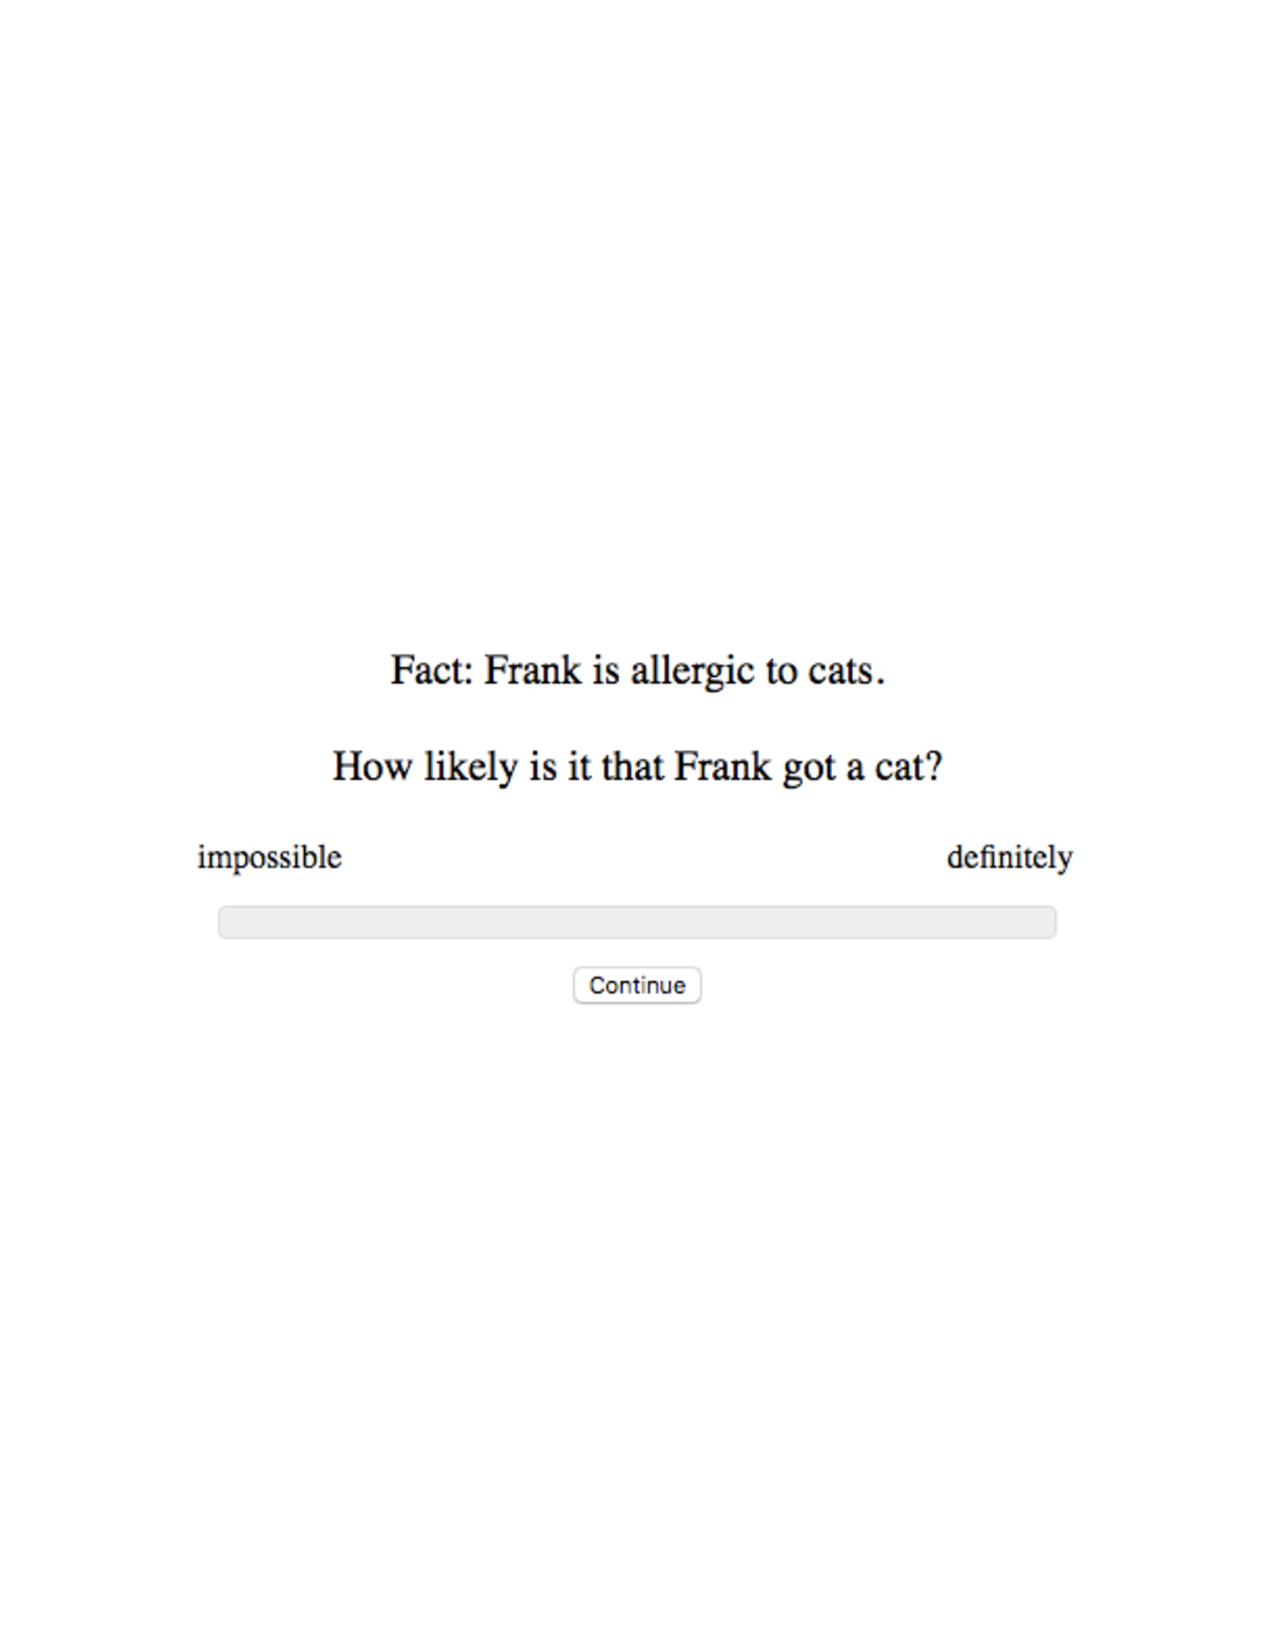
\includegraphics[width=8cm]{figures/exp1-trial}}
\end{center}
\caption{A sample trial in the prior probability norming study}\label{f-trial-exp1}
\end{figure}

After completing the experiment, participants filled out a short optional survey about their age, their gender, their native language(s) and, if English is their native language, whether they are a speaker of American English (as opposed to, e.g., Australian or Indian English). To encourage them to respond truthfully, participants were told that they would be paid no matter what answers they gave in the survey. 

\paragraph{Data exclusion.}
Prior to analysis, the data from 8 participants who did not self-identify as native speakers of American English were excluded. For the remaining 87 participants, we inspected their responses to the two control stimuli (the group means were .86 for (\ref{control1}) and .03 for (\ref{control2})). 19 participants gave responses lower than .8 to (\ref{control1}) or responses higher than .2 to (\ref{control2}), suggesting that these participants did not attend to the task or interpreted the task differently. The data from these 19 participants were also excluded, leaving data from 68 participants (ages 21-75; median: 36; 31 female, 37 male).  



\subsection{Results and discussion}

As expected, likeliness ratings of events were influenced by facts about the world: overall, the mean likeliness rating for events presented with facts that make the event more likely was .7 (sd = .21) and the mean likeliness rating for events presented with facts that make the event less likely was .16 (sd = .17). Figure \ref{f-priors} shows the likeliness rating for the 20 events given facts that make the events more likely (brown dots) and facts that make the events less likely (blue dots). Mean likeliness ratings for each of the 40 fact/event pairs are shown as black dots. Error bars indicate 95\% confidence intervals.

\begin{figure}
\centering

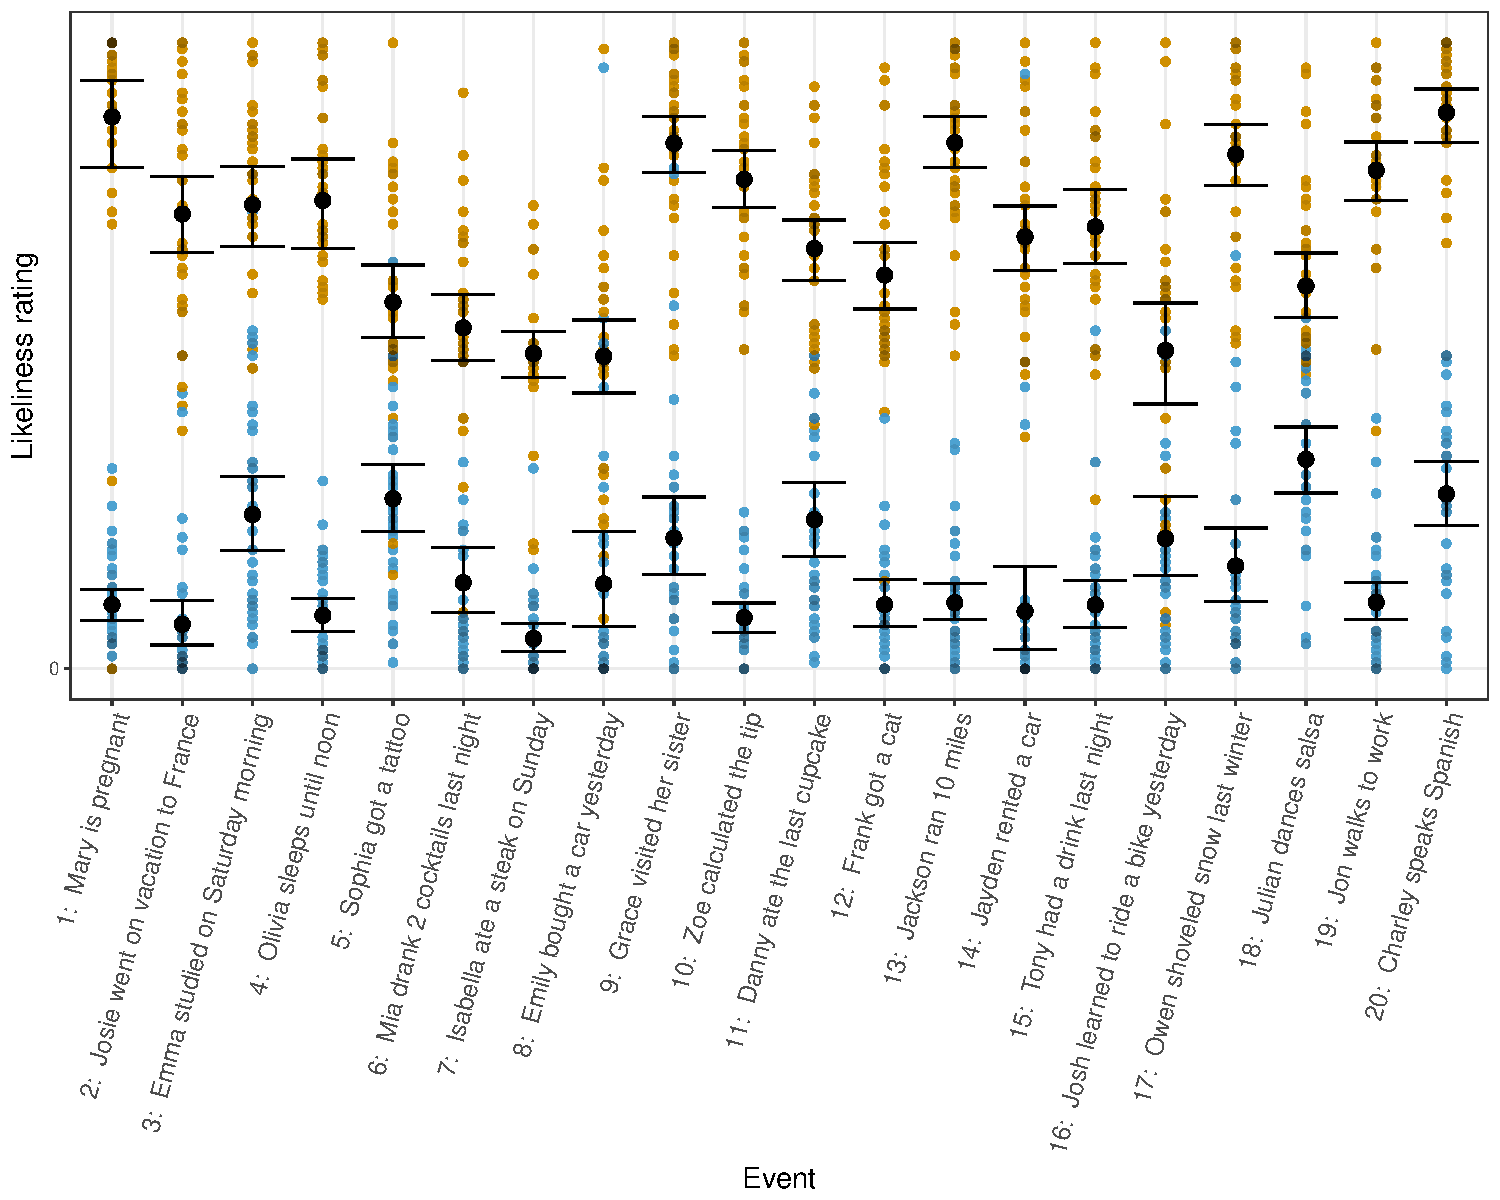
\includegraphics[width=.8\paperwidth]{../results/1-prior/graphs/target-ratings}

\caption{Likeliness ratings for 20 events given facts about the world that make the events more likely (brown dots) and facts about the world that make the events less likely (blue dots); darker dots indicate overlapping ratings. Mean likeliness ratings for the 40 fact/event pairs are given by black dots. Error bars indicate 95\% confidence intervals.}\label{f-priors}
\end{figure}

For each event, the likeliness of the event is higher given the fact that makes the event more likely than given the fact that makes the event less likely. At the same time, the likeliness of none of the events given a particular fact is at ceiling or at floor. We have thus succeeded in identifying suitable fact/fact/event triples for our study of how projectivity is influenced by event probability.

\section{Veridicality}\label{s-norming2}

\subsection{Methods}\label{s-methods-2}

\paragraph{Participants.} 300 participants with U.S.\ IP addresses and at least 99\% of previous HITs approved were recruited on Amazon's Mechanical Turk platform (ages: 19-73, median: 33; 127 female, 169 male, 2 other, 2 didn't provide information). They were paid 75 cents for participating in the experiment.

\paragraph{Materials.} The veridicality of 20 predicates was explored in this experiment: {\em be annoyed, know, discover, reveal, see, establish, pretend, think, suggest, prove, demonstrate, say, hear, confess, inform, announce, acknowledge, admit, confirm} and {\em be right}. 

{\bf include info on why these were included}

400 sentences were formed by combining the 20 predicates with a (random) proper name subject and a complement clause that lexicalized one of the 20 events explored in the prior probability norming study described in section \ref{s-norming1} (see Appendix \ref{a-exp1}).\footnote{past tense, present tense, inform Sam} The target stimuli consisted of one of these 400 sentences followed by a {\em but I know that}-clause that denied the truth of the complement clause, as shown in the sample stimuli in (\ref{stims}). The speaker of the target stimuli was realized by a (bold-faced) proper name. The proper names that realized the speakers and the subjects of the 20 predicates, and that occurred in the complement clauses were all unique. The gender of the proper name subject of the predicate was distinct from the gender of the proper name in the complement clause, to ensure that the pronoun in the {\em but I know that}-clause unambiguously referred to the person referred to in the complement clause of the predicate.

\begin{exe}
\ex\label{stims}
\begin{xlist}
\ex {\bf Christopher:} Melissa knows that Danny ate the last cupcake, but I know that he didn't.
\ex {\bf Susan:} Jerry pretended that Emma studied on Saturday morning, but I know that she didn't.
\end{xlist}
\end{exe}

The experiment also included eight control stimuli, which were used to assess whether participants were attending to the task. The four control stimuli in (\ref{control-good}) were hypothesized to be non-contradictory, and the four control stimuli in (\ref{control-bad}) were hypothesized to be contradictory.

\begin{exe}
\ex\label{control-good}
\begin{xlist}
\ex Zack believes that I'm married, but I'm actually single.
\ex Tara wants me to cook for her and I'm a terrific cook.
\ex Frederick is both smarter and taller than I am.
\ex Vanessa is really good at math, but I'm not.
\end{xlist}
\ex\label{control-bad}
\begin{xlist}
\ex Dana has never smoked in her life and she stopped smoking recently.
\ex Hendrick's car is completely red and his car is not red.
\ex Madison laughed loudly and she didn't laugh.
\ex Sebastian lives in the USA and has never been to the USA.
\end{xlist}
\end{exe}

Each participant saw a random set of 28 stimuli: each set contained one stimulus for each of the 20 predicates (each with a unique complement clause) and the same 8 control stimuli. Trial order was randomized.

\paragraph{Procedure.} Participants were told that they would read utterances made by a speaker and were asked to assess whether the speaker's utterance is contradictory. On each trial, participants read the speaker's utterance and then gave their response on a slider marked `definitely no' at one end (coded as 0) and `definitely yes' at the other (coded as 1), as shown in Figure \ref{f-trial-exp2}.   

\begin{figure}[h!]
\begin{center}
\fbox{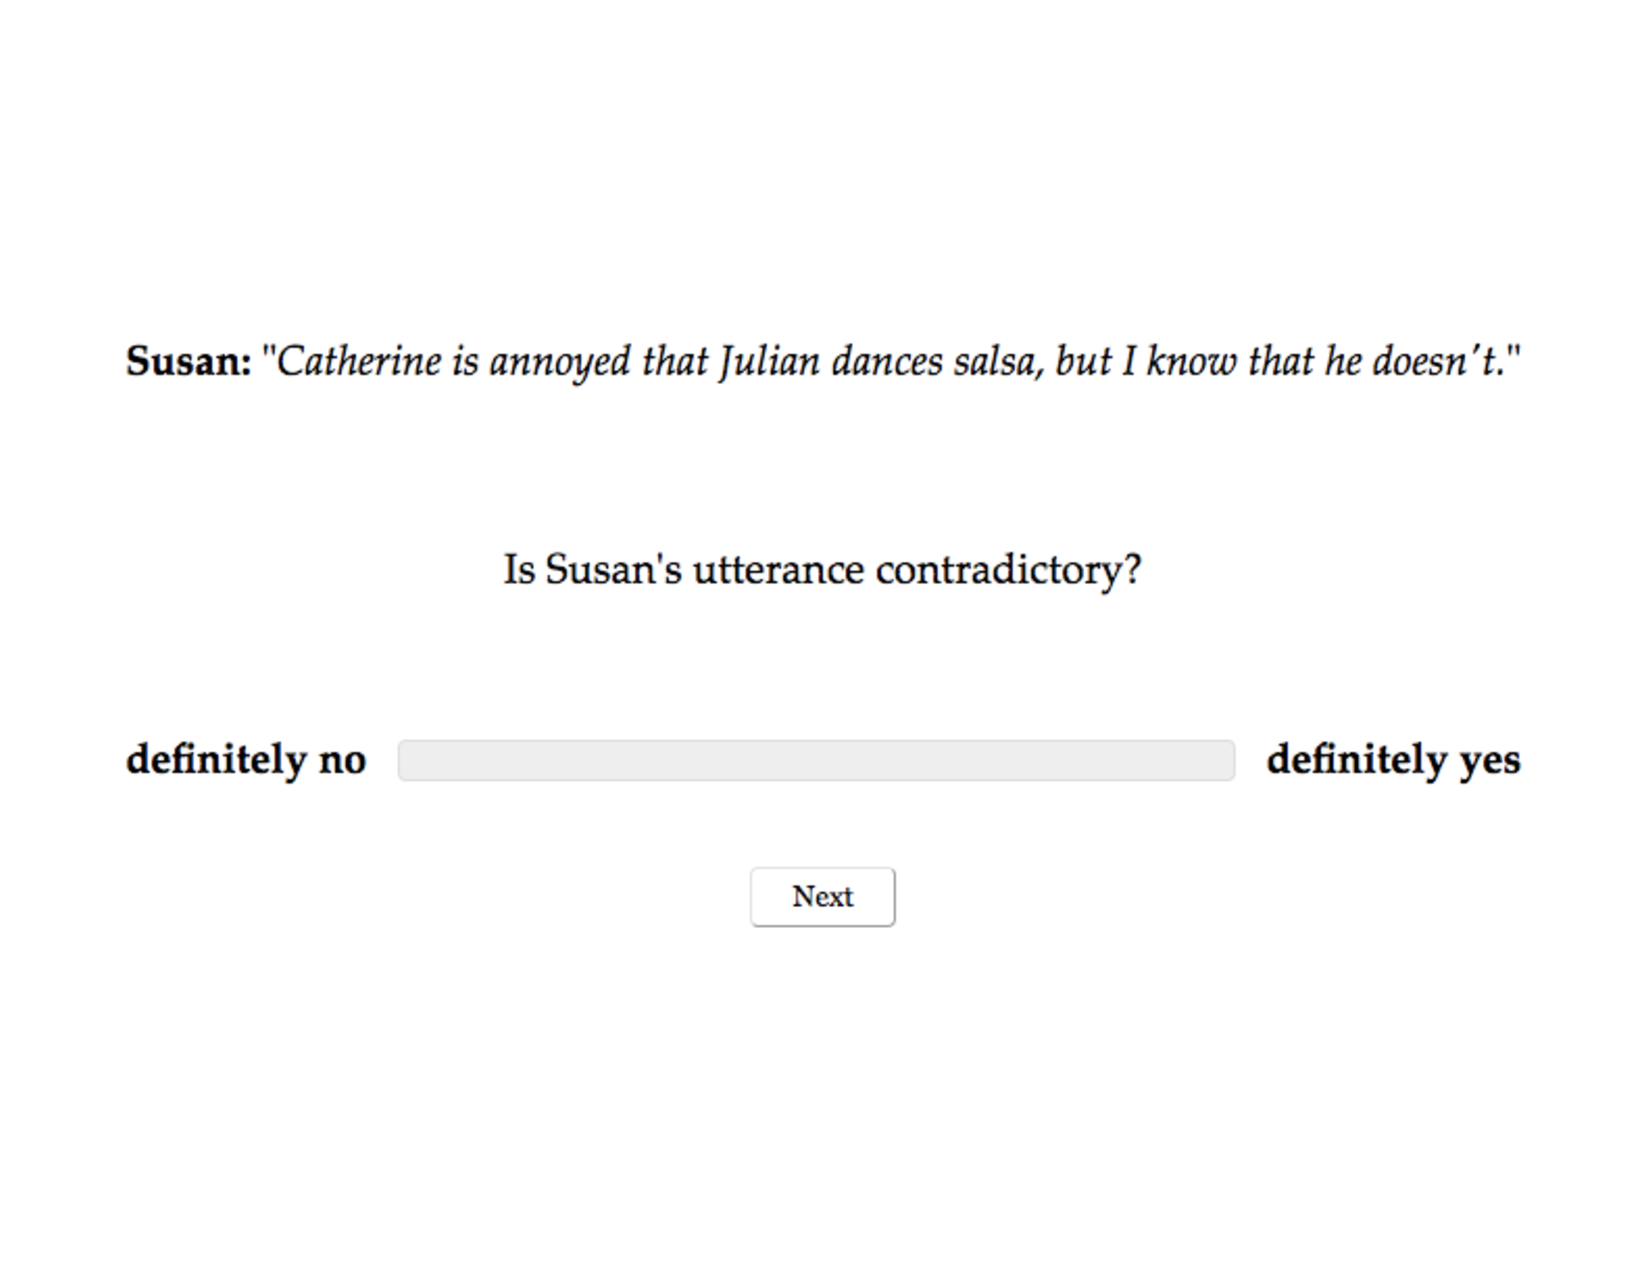
\includegraphics[width=10cm]{figures/exp2-trial}}
\end{center}
\caption{A sample trial in in the veridicality norming study}\label{f-trial-exp2}
\end{figure}

After completing the experiment, participants filled out a short, optional survey about their age, their gender, their native language(s) and, if English is their native language, whether they are a speaker of American English (as opposed to, e.g., Australian or Indian English). To encourage them to respond truthfully, participants were told that they would be paid no matter what answers they gave in the survey.

\paragraph{Data exclusion.}
Prior to analysis, the data from 14 participants who did not self-identify as native speakers of American English were excluded. For the remaining 286 participants, we inspected their responses to the 8 control stimuli: we expected low responses to the non-contradictory stimuli in (\ref{control-good}) and high responses to the contradictory stimuli in (\ref{control-bad}). The response means of 11 participants were more than 3 standard deviations above the group mean for the non-contradictory control stimuli or below the group mean for the contradictory control stimuli (the group means were .15 and .92, respectively).\footnote{The response mean of one of the non-contradictory control stimuli, (\ref{control-good}a) {\em Zack believes that I'm married, but I'm actually single}, was higher, at .36, than the response means of the remaining three non-contradictory control stimuli (which were .06, .07 and .09, respectively). We hypothesize that some participants gave a higher response to this stimulus because the speaker can be taken to contradict Zack's belief. If responses to this control stimulus are not considered, then the response means of an additional four participants are more than 3 standard deviations above the group response mean for the remaining three non-contradictory control stimuli (with the group mean at .08). {\bf SAY WHETHER ANYTHING IN ANALYSIS CHANGES IF WE DO SO.}} Closer inspection revealed that these participants' responses to the control stimuli were systematically higher or lower, suggesting that these participants did not attend to the task or interpreted the task differently. The data from these 11 participants were also excluded, leaving data from 275 participants (ages 19-73; median: 35; 119 female, 153 male, 2 other, 1 didn't provide information).  

\subsection{Results}

Figure \ref{f-veridicality-predicate} shows the contradictoriness ratings by predicate, collapsing over the 20 complement clauses that each predicate was paired with. As expected, the five predicates that do not entail the content of the complement, namely {\em pretend, suggest, think, hear} and {\em say}, have the lowest mean contradictoriness ratings. Furthermore, the predicate {\em be right} has the highest mean contradictoriness rating, thereby confirming the assumption that the content of its clausal complement is entailed. 


\begin{figure}[h!]
\centering

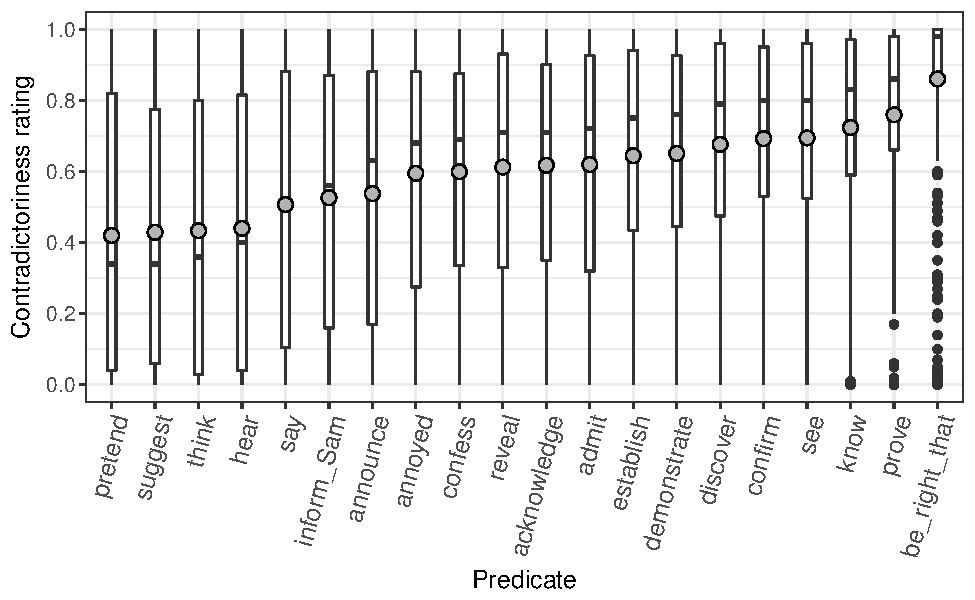
\includegraphics[width=.8\paperwidth]{../results/2-veridicality/graphs/boxplot-veridicality}

\caption{Boxplot of contradictoriness ratings by predicate, collapsing across complement clauses. Grey dots indicate means and notches indicate medians.}
\label{f-veridicality-predicate}
\end{figure}

\begin{figure}[h!]
\centering

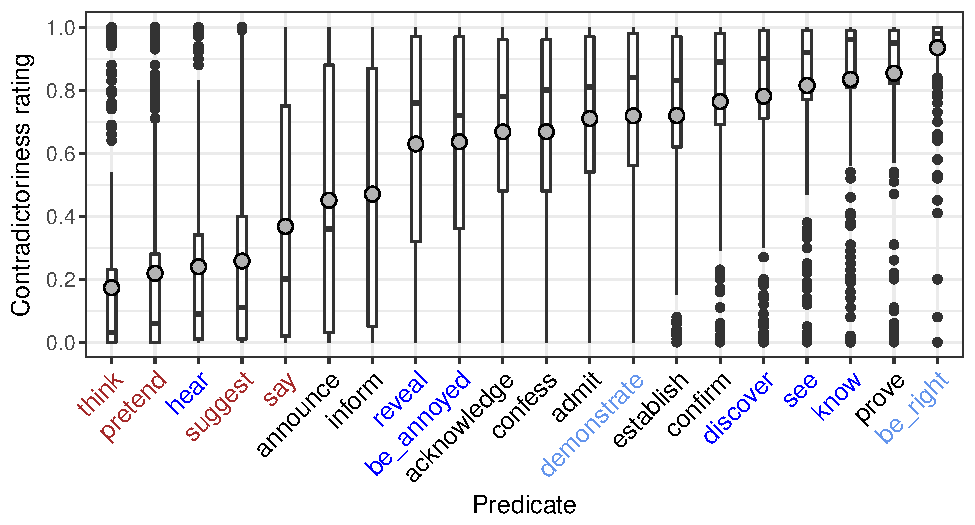
\includegraphics[width=.8\paperwidth]{../results/2-veridicality2/graphs/boxplot-veridicality}

\caption{Boxplot of contradictoriness ratings by predicate, collapsing across complement clauses. Grey dots indicate means and notches indicate medians.}
\label{f-veridicality-predicate}
\end{figure}

\newpage

To determine which predicates differed from each other in veridicality, we conducted post hoc pairwise comparisons using Tukey's method (allowing for by-participant variability), using the \verb|lsmeans| package \citep{tukey} in R \citep{r}. P-values for each pair of predicates are displayed in Table \ref{t-pairwise}. The color-coding of table columns indicates the standard assumptions about whether the content of the complement is entailed: predicates written in brown font are typically taken to not entail the content of the complement, predicates written in blue font are typically taken to entail the content of the complement, and predicates written in green font have been discussed as being easily taken to entail but don't really entail.

These results confirm commonly-made assumptions about entailment. First, the five predicates that are typically taken to not entail the content of the complement ({\em pretend, suggest, think, hear, say}) received significantly lower contradictoriness ratings than the seven predicates that are typically taken to entail the content of the complement ({\em annoyed, know, discover, reveal, see, establish, be right}). Furthermore, these results suggest that, of the five predicates that are typically assumed to not entail the content of the complement, all but {\em say} are significantly less veridical than {\em inform}, the least veridical of the entailed? predicates.

The results suggest no differences in the veridicality of the verbs of saying, {\em say, inform} and {\em announce}. The next set of predicates for which the results suggest no difference in veridicality consists of {\em be annoyed, confess, reveal, acknowledge} and {\em demonstrate}. This set of predicates consists both of predicates for which the content of the complement is typically taken to be entailed (e.g., {\em be annoyed}) and of predicates for which the content of the complement is not really entailed (e.g., {\em confess}). The next set consists of {\em discover, confirm} and {\em see}. Finally, {\em know} and {\em prove}, which are indistinguishable, and {\em be right}, which is significantly more veridical than all other predicates.

\begin{landscape}
\begin{table}[h!]
\centering
\begin{tabular}{l l l l l l l l l l l l l l l l l l l l }
\toprule

 &   \rot{{\em pretend}} & \rot{{\em suggest}} & \rot{{\em think}} &  \rot{{\em hear}} &  \rot{{\em say}} & \rot{{\em inform}} & \rot{{\em announce}} & \rot{{\em annoyed}} & \rot{{\em confess}} & \rot{{\em reveal}} & \rot{{\em acknowledge}} & \rot{{\em admit}} & \rot{{\em establish}}  & \rot{{\em demonstrate}}  & \rot{{\em discover}}  & \rot{{\em confirm}} & \rot{{\em see}}  & \rot{{\em know}}  & \rot{{\em prove}}  \\
\midrule
\color{brown}{\em pretend}\color{black}		& - & - & - & - & - & - & - & - & - & - & - & - & - & - & - & - & - & - & - \\
\color{brown}{\em suggest}\color{black}		& n.s. & - & - & - & - & - & - & - & - & - & - & - & - & - & - & - & - & - & - \\
\color{brown}{\em think}\color{black}			& n.s. & n.s. & - & - & - & - & - & - & - & - & - & - & - & - & - & - & - & - & - \\
\color{brown}{\em hear}	\color{black}		& n.s. & n.s. & n.s. & - & - & - & - & - & - & - & - & - & - & - & - & - & - & - & - \\
\color{brown}{\em say}\color{black}		& ** & ** & * & . & - & - & - & - & - & - & - & - & - & - & - & - & - & - & - \\
\color{green}{\em inform}\color{black}		& *** & *** & *** & ** & n.s. & - & - & - & - & - & - & - & - & - & - & - & - & - & - \\
\color{green}{\em announce}\color{black}		& *** & *** & *** & *** & n.s. & n.s. & - & - & - & - & - & - & - & - & - & - & - & - & - \\
\color{blue}{\em annoyed}\color{black}		& *** & *** & *** & *** & *** & * & n.s. & - & - & - & - & - & - & - & - & - & - & - & - \\
\color{green}{\em confess}\color{black}		& *** & *** & *** & *** & *** & * & n.s. & n.s. & - & - & - & - & - & - & - & - & - & - & - \\
\color{blue}{\em reveal}\color{black}		& *** & *** & *** & *** & *** & ** & * & n.s. & n.s. & - & - & - & - & - & - & - & - & - & - \\
\color{green}{\em acknowledge}\color{black}	& *** & *** & *** & *** & *** & *** & ** & n.s. & n.s. & n.s. & - & - & - & - & - & - & - & - & - \\
\color{green}{\em admit}\color{black}			& *** & *** & *** & *** & *** & *** & ** & n.s. & n.s. & n.s. & n.s. & - & - & - & - & - & - & - & - \\
\color{blue}{\em establish}\color{black}		& *** & *** & *** & *** & *** & *** & *** & n.s. & n.s. & n.s. & n.s. &  n.s. & - & - & - & - & - & - & - \\
\color{green}{\em demonstrate}\color{black}	& *** & *** & *** & *** & *** & *** & *** & n.s. & n.s. & n.s. & n.s. & n.s. & n.s. & - & - & - & - & - & - \\
\color{blue}{\em discover}\color{black}		& *** & *** & *** & *** & *** & *** & *** & ** & ** & . & n.s. & n.s. & n.s. & n.s. & - & - & - & - & - \\
\color{green}{\em confirm}\color{black}		& *** & *** & *** & *** & *** & *** & *** & *** & *** & ** & * & * & n.s. & n.s. & n.s. & - & - & - & - \\
\color{blue}{\em see}\color{black}			& *** & *** & *** & *** & *** & *** & *** & *** & *** & ** & ** & * & n.s. & n.s. & n.s. & n.s. & - & - & - \\
\color{blue}{\em know}\color{black}			& *** & *** & *** & *** & *** & *** & *** & *** & *** & *** & *** & *** & ** & * & n.s. & n.s. & n.s. & - & - \\
\color{green}{\em prove}\color{black}			& *** & *** & *** & *** & *** & *** & *** & *** & *** & *** & *** & *** & *** & *** & ** & . & . & n.s. & -  \\
\color{blue}{\em be right}\color{black}		& *** & *** & *** & *** & *** & *** & *** & *** & ***  & ***  & *** & *** & *** & *** & *** & *** & *** & *** & ***  \\

\bottomrule
\end{tabular}
\caption{P-values associated with pairwise comparison of contraditoriness ratings of prediates using Tukey's method. `***' indicates significance at .001, `**' at .01, `*' at .05, `.' marginal significance at .1, and `n.s' indicates no significant difference in means.}\label{t-pairwise}
\end{table}
\end{landscape}

\newpage

\begin{landscape}
\begin{table}[h!]
\centering
\begin{tabular}{l l l l l l l l l l l l l l l l l l l l }
\toprule

 &   \rot{{\em think}} & \rot{{\em pretend}} & \rot{{\em hear}} &  \rot{{\em suggest}} &  \rot{{\em say}} & \rot{{\em announce}} & \rot{{\em inform}} & \rot{{\em reveal}} & \rot{{\em be annoyed}} & \rot{{\em confess}} & \rot{{\em acknowledge}} & \rot{{\em admit}} & \rot{{\em establish}}  & \rot{{\em demonstrate}}  & \rot{{\em confirm}}  & \rot{{\em discover}} & \rot{{\em see}}  & \rot{{\em know}}  & \rot{{\em prove}}  \\
\midrule
\color{brown}{\em think}\color{black}		& -- & - & - & - & - & - & - & - & - & - & - & - & - & - & - & - & - & - & - \\
\color{brown}{\em pretend}\color{black}		& n.s. & - & - & - & - & - & - & - & - & - & - & - & - & - & - & - & - & - & - \\
\color{brown}{\em hear}\color{black}			& n.s. & n.s. & - & - & - & - & - & - & - & - & - & - & - & - & - & - & - & - & - \\
\color{brown}{\em suggest}	\color{black}		& * & n.s. & n.s. & - & - & - & - & - & - & - & - & - & - & - & - & - & - & - & - \\
\color{brown}{\em say}\color{black}		& *** & *** & *** & *** & - & - & - & - & - & - & - & - & - & - & - & - & - & - & - \\
\color{green}{\em announce}\color{black}		& *** & *** & *** & *** & * & - & - & - & - & - & - & - & - & - & - & - & - & - & - \\
\color{green}{\em inform}\color{black}		& *** & *** & *** & *** & *** & n.s. & - & - & - & - & - & - & - & - & - & - & - & - & - \\
\color{blue}{\em reveal}\color{black}		& *** & *** & *** & *** & *** & *** & *** & - & - & - & - & - & - & - & - & - & - & - & - \\
\color{blue}{\em be annoyed}\color{black}		& *** & *** & *** & *** & *** & *** & *** & n.s. & - & - & - & - & - & - & - & - & - & - & - \\
\color{green}{\em confess}\color{black}		& *** & *** & *** & *** & *** & *** & *** & n.s. & n.s. & - & - & - & - & - & - & - & - & - & - \\
\color{green}{\em acknowledge}\color{black}	& *** & *** & *** & *** & *** & *** & *** & n.s. & n.s. & n.s. & - & - & - & - & - & - & - & - & - \\
\color{green}{\em admit}\color{black}			& *** & *** & *** & *** & *** & *** & *** & * & . & n.s. & n.s. & - & - & - & - & - & - & - & - \\
\color{blue}{\em establish}\color{black}		& *** & *** & *** & *** & *** & *** & *** & ** & * & n.s. & n.s. &  n.s. & - & - & - & - & - & - & - \\
\color{green}{\em demonstrate}\color{black}	& *** & *** & *** & *** & *** & *** & *** & ** & * & n.s. & n.s. & n.s. & n.s. & - & - & - & - & - & - \\
\color{green}{\em confirm}\color{black}		& *** & *** & *** & *** & *** & *** & *** & *** & *** & ** & ** & n.s. & n.s. & n.s. & - & - & - & - & - \\
\color{blue}{\em discover}\color{black}		& *** & *** & *** & *** & *** & *** & *** & *** & *** & *** & *** & n.s. & n.s. & n.s. & n.s. & - & - & - & - \\
\color{blue}{\em see}\color{black}			& *** & *** & *** & *** & *** & *** & *** & *** & *** & *** & *** & *** & ** & ** & n.s. & n.s. & - & - & - \\
\color{blue}{\em know}\color{black}			& *** & *** & *** & *** & *** & *** & *** & *** & *** & *** & *** & *** & *** & *** & n.s. & n.s. & n.s. & - & - \\
\color{green}{\em prove}\color{black}			& *** & *** & *** & *** & *** & *** & *** & *** & *** & *** & *** & *** & *** & *** & ** & n.s. & n.s. & n.s. & -  \\
\color{blue}{\em be right}\color{black}		& *** & *** & *** & *** & *** & *** & *** & *** & ***  & ***  & *** & *** & *** & *** & *** & *** & *** & *** & *  \\

\bottomrule
\end{tabular}
\caption{{\bf RESULTS FROM NEW RUN OF EXPERIMENT} P-values associated with pairwise comparison of contraditoriness ratings of prediates using Tukey's method. `***' indicates significance at .001, `**' at .01, `*' at .05, `.' marginal significance at .1, and `n.s' indicates no significant difference in means.}\label{t-pairwise}
\end{table}
\end{landscape}


\newpage

Significant differences for restricted set:

\begin{itemize}

\item The five predicates that are typically taken to not entail the content of the complement (`no': {\em pretend, suggest, think, hear, say}) received significantly lower contradictoriness ratings than the seven predicates that are typically taken to entail the content of the complement ({\em annoyed, know, discover, reveal, see, establish, be right}). {\bf except that now say is not different from annoyed}

\item {\em inform (no?)} is still least veridical of the no?/yes predicates, next is {\em announce (no?)}: `no' predicates {\em suggest} and {\em pretend} are less veridical than {\em inform} and {\em announce}, {\em think} and {\em hear} are only less veridical than {\em announce}

\item The results suggest no differences in the veridicality of the verbs of communication, {\em say, inform} and {\em announce}. 

\item Highest veridicality, indistinguishable: {\em see, discover, prove (no?), confirm (no?), be right, know}, all have medians at ceiling

\item {\em confess (no?), reveal (yes), admit (no?), acknowledge (no?), establish (yes), demonstrate (no?)} are indistinguishable the highest veridicality verbs except {\em know}, so probably also indistinguishable from {\em know}.

\item {\em annoyed} is more veridical than {\em hear} and less veridical than {\em discover}, i.e., indistinguishable from {\em say, inform, announce, confess, reveal, admit acknowledge, establish, demonstrate, see}

\end{itemize}

%# suggest - inform_Sam        -0.131375 0.03818901 1520  -3.440  0.0708
%# suggest - announce          -0.158250 0.03818901 1520  -4.144  0.0057
%# suggest - annoyed           -0.190625 0.03818901 1520  -4.992  0.0001
%# suggest - confess           -0.259125 0.03818901 1520  -6.785  <.0001
%# suggest - reveal            -0.262625 0.03818901 1520  -6.877  <.0001
%# suggest - admit             -0.265750 0.03818901 1520  -6.959  <.0001
%# suggest - acknowledge       -0.279875 0.03818901 1520  -7.329  <.0001
%# suggest - establish         -0.283750 0.03818901 1520  -7.430  <.0001
%# suggest - demonstrate       -0.287500 0.03818901 1520  -7.528  <.0001
%# suggest - see               -0.308250 0.03818901 1520  -8.072  <.0001
%# suggest - discover          -0.344250 0.03818901 1520  -9.014  <.0001
%# suggest - prove             -0.344500 0.03818901 1520  -9.021  <.0001
%# suggest - confirm           -0.364750 0.03818901 1520  -9.551  <.0001
%# suggest - be_right_that     -0.383250 0.03818901 1520 -10.036  <.0001
%# suggest - know              -0.431375 0.03818901 1520 -11.296  <.0001
%
%
%# pretend - inform_Sam        -0.129750 0.03818901 1520  -3.398  0.0805
%# pretend - announce          -0.156625 0.03818901 1520  -4.101  0.0068
%# pretend - annoyed           -0.189000 0.03818901 1520  -4.949  0.0001
%# pretend - confess           -0.257500 0.03818901 1520  -6.743  <.0001
%# pretend - reveal            -0.261000 0.03818901 1520  -6.834  <.0001
%# pretend - admit             -0.264125 0.03818901 1520  -6.916  <.0001
%# pretend - acknowledge       -0.278250 0.03818901 1520  -7.286  <.0001
%# pretend - establish         -0.282125 0.03818901 1520  -7.388  <.0001
%# pretend - demonstrate       -0.285875 0.03818901 1520  -7.486  <.0001
%# pretend - see               -0.306625 0.03818901 1520  -8.029  <.0001
%# pretend - discover          -0.342625 0.03818901 1520  -8.972  <.0001
%# pretend - prove             -0.342875 0.03818901 1520  -8.978  <.0001
%# pretend - confirm           -0.363125 0.03818901 1520  -9.509  <.0001
%# pretend - be_right_that     -0.381625 0.03818901 1520  -9.993  <.0001
%# pretend - know              -0.429750 0.03818901 1520 -11.253  <.0001
%
%
%# think - announce            -0.142375 0.03818901 1520  -3.728  0.0274
%# think - annoyed             -0.174750 0.03818901 1520  -4.576  0.0009
%# think - confess             -0.243250 0.03818901 1520  -6.370  <.0001
%# think - reveal              -0.246750 0.03818901 1520  -6.461  <.0001
%# think - admit               -0.249875 0.03818901 1520  -6.543  <.0001
%# think - acknowledge         -0.264000 0.03818901 1520  -6.913  <.0001
%# think - establish           -0.267875 0.03818901 1520  -7.014  <.0001
%# think - demonstrate         -0.271625 0.03818901 1520  -7.113  <.0001
%# think - see                 -0.292375 0.03818901 1520  -7.656  <.0001
%# think - discover            -0.328375 0.03818901 1520  -8.599  <.0001
%# think - prove               -0.328625 0.03818901 1520  -8.605  <.0001
%# think - confirm             -0.348875 0.03818901 1520  -9.135  <.0001
%# think - be_right_that       -0.367375 0.03818901 1520  -9.620  <.0001
%# think - know                -0.415500 0.03818901 1520 -10.880  <.0001
%
%
%# hear - announce             -0.134000 0.03818901 1520  -3.509  0.0571
%# hear - annoyed              -0.166375 0.03818901 1520  -4.357  0.0023
%# hear - confess              -0.234875 0.03818901 1520  -6.150  <.0001
%# hear - reveal               -0.238375 0.03818901 1520  -6.242  <.0001
%# hear - admit                -0.241500 0.03818901 1520  -6.324  <.0001
%# hear - acknowledge          -0.255625 0.03818901 1520  -6.694  <.0001
%# hear - establish            -0.259500 0.03818901 1520  -6.795  <.0001
%# hear - demonstrate          -0.263250 0.03818901 1520  -6.893  <.0001
%# hear - see                  -0.284000 0.03818901 1520  -7.437  <.0001
%# hear - discover             -0.320000 0.03818901 1520  -8.379  <.0001
%# hear - prove                -0.320250 0.03818901 1520  -8.386  <.0001
%# hear - confirm              -0.340500 0.03818901 1520  -8.916  <.0001
%# hear - be_right_that        -0.359000 0.03818901 1520  -9.401  <.0001
%# hear - know                 -0.407125 0.03818901 1520 -10.661  <.0001
%
%# say - confess               -0.136000 0.03818901 1520  -3.561  0.0482
%# say - reveal                -0.139500 0.03818901 1520  -3.653  0.0356
%# say - admit                 -0.142625 0.03818901 1520  -3.735  0.0268
%# say - acknowledge           -0.156750 0.03818901 1520  -4.105  0.0067
%# say - establish             -0.160625 0.03818901 1520  -4.206  0.0044
%# say - demonstrate           -0.164375 0.03818901 1520  -4.304  0.0029
%# say - see                   -0.185125 0.03818901 1520  -4.848  0.0002
%# say - discover              -0.221125 0.03818901 1520  -5.790  <.0001
%# say - prove                 -0.221375 0.03818901 1520  -5.797  <.0001
%# say - confirm               -0.241625 0.03818901 1520  -6.327  <.0001
%# say - be_right_that         -0.260125 0.03818901 1520  -6.812  <.0001
%# say - know                  -0.308250 0.03818901 1520  -8.072  <.0001
%
%
%# inform_Sam - confess        -0.127750 0.03818901 1520  -3.345  0.0940
%# inform_Sam - reveal         -0.131250 0.03818901 1520  -3.437  0.0715
%# inform_Sam - admit          -0.134375 0.03818901 1520  -3.519  0.0553
%# inform_Sam - acknowledge    -0.148500 0.03818901 1520  -3.889  0.0154
%# inform_Sam - establish      -0.152375 0.03818901 1520  -3.990  0.0105
%# inform_Sam - demonstrate    -0.156125 0.03818901 1520  -4.088  0.0071
%# inform_Sam - see            -0.176875 0.03818901 1520  -4.632  0.0007
%# inform_Sam - discover       -0.212875 0.03818901 1520  -5.574  <.0001
%# inform_Sam - prove          -0.213125 0.03818901 1520  -5.581  <.0001
%# inform_Sam - confirm        -0.233375 0.03818901 1520  -6.111  <.0001
%# inform_Sam - be_right_that  -0.251875 0.03818901 1520  -6.595  <.0001
%# inform_Sam - know           -0.300000 0.03818901 1520  -7.856  <.0001
%
%
%# announce - demonstrate      -0.129250 0.03818901 1520  -3.384  0.0837
%# announce - see              -0.150000 0.03818901 1520  -3.928  0.0133
%# announce - discover         -0.186000 0.03818901 1520  -4.871  0.0002
%# announce - prove            -0.186250 0.03818901 1520  -4.877  0.0002
%# announce - confirm          -0.206500 0.03818901 1520  -5.407  <.0001
%# announce - be_right_that    -0.225000 0.03818901 1520  -5.892  <.0001
%# announce - know             -0.273125 0.03818901 1520  -7.152  <.0001
%
%# annoyed - discover          -0.153625 0.03818901 1520  -4.023  0.0092
%# annoyed - prove             -0.153875 0.03818901 1520  -4.029  0.0090
%# annoyed - confirm           -0.174125 0.03818901 1520  -4.560  0.0010
%# annoyed - be_right_that     -0.192625 0.03818901 1520  -5.044  0.0001
%# annoyed - know              -0.240750 0.03818901 1520  -6.304  <.0001
%
%# confess - know              -0.172250 0.03818901 1520  -4.510  0.0012
%# reveal - know               -0.168750 0.03818901 1520  -4.419  0.0018
%# admit - know                -0.165625 0.03818901 1520  -4.337  0.0025
%# acknowledge - know          -0.151500 0.03818901 1520  -3.967  0.0114
%# establish - know            -0.147625 0.03818901 1520  -3.866  0.0167
%# demonstrate - know          -0.143875 0.03818901 1520  -3.767  0.0239

\newpage

\begin{figure}[h!]
\centering


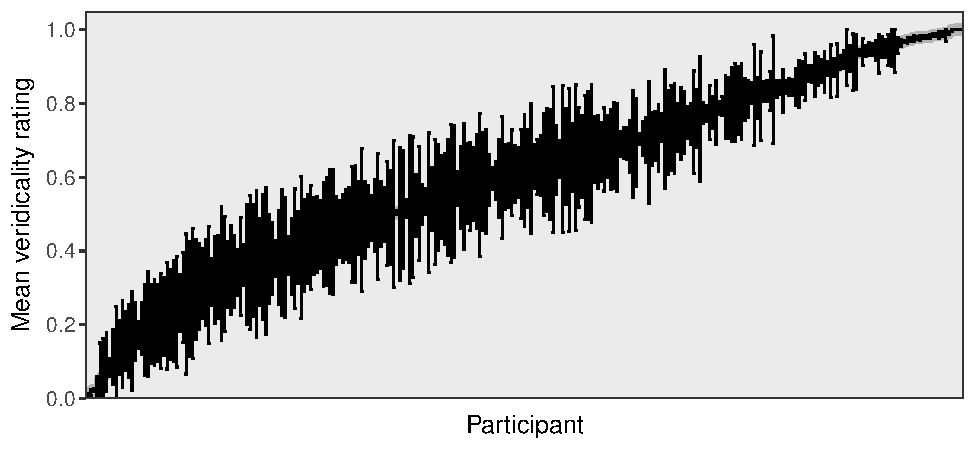
\includegraphics[width=12cm]{../results/2-veridicality/graphs/veridicality-subjmeans}
	

\caption{Boxplot of contradictoriness ratings by participant, collapsing across predicates and complement clauses. Grey dots indicate means and error bars indicate bootstrapped 95\% confidence intervals.}
\label{}
\end{figure}

\subsection{Discussion}

\subsection{Interim summary}

\section{Projectivity}

\section{Discussion}

\section{Conclusions}\label{s6}


\appendix

\setcounter{table}{0}
\renewcommand{\thetable}{A\arabic{table}}

\setcounter{figure}{0}
\renewcommand{\thefigure}{A\arabic{figure}}

\section{Materials used in the event probability norming study}\label{a-exp1}

The 20 event descriptions used in the event probability pretest; facts about the world that make the event more (H) or less likely (L) are given in parentheses. 

\begin{enumerate}[leftmargin=3ex,itemsep=-2pt]
\item Mary is pregnant (Mary is a middle school student / Mary is taking a prenatal yoga class)
\item Josie went on vacation to France (Josie doesn't have a passport / Josie loves France)
\item Emma studied on Saturday morning (Emma is in first grade / Emma is in law school)
\item Olivia sleeps until noon (Olivia has two small children / Olivia works the third shift)
\item Sophia got a tattoo (Sophia is a high end fashion model / Sophia is a hipster)
\item Mia drank 2 cocktails last night (Mia is a nun / Mia is a college student)
\item Isabella ate a steak on Sunday (Isabella is a vegetarian / Isabella is from Argentina)
\item  Emily bought a car yesterday (Emily never has any money / Emily has been saving for a year)
\item  Grace visited her sister (Grace hates her sister / Grace loves her sister)
\item Zoe calculated the tip (Zoe is 5 years old / Zoe is a math major)
\item  Danny ate the last cupcake (Danny is a diabetic / Danny loves cake)
\item  Frank got a cat (Frank is allergic to cats / Frank has always wanted a pet)
\item  Jackson ran 10 miles (Jackson is obese / Jackson is training for a marathon)
\item  Jayden rented a car (Jayden doesn't have a driver's license / Jayden's car is in the shop)
\item  Tony had a drink last night (Tony has been sober for 20 years / Tony really likes to party with his friends)
\item  Josh learned to ride a bike yesterday (Josh is a 75-year old man / Josh is a 5-year old boy)
\item  Owen shoveled snow last winter (Owen lives in New Orleans / Owen lives in Chicago)
\item  Julian dances salsa (Julian is German / Julian is Cuban)
\item  Jon walks to work (Jon lives 10 miles away from work / Jon lives 2 blocks away from work)
\item  Charley speaks Spanish (Charley lives in Korea / Charley lives in Mexico)
\end{enumerate}

\clearpage

\section{Materials used in Exp 2}\label{a-exp2}

\section{Materials used in Exp 3}\label{a-exp3}

\bibliographystyle{cslipubs-natbib}
\bibliography{bibliography}


\end{document}
